For some applications segmenting an image is not enough, as it may be important to know what each segmented region present. The aim of segmentation is just to partition a given image into regions, without giving information on what these regions mean. The more complication task of assigning meaning to image regions is named semantic segmentation. It goes a step further into understanding an image, as apart from dividing an image into regions, which correspond to objects, it also recognises what those regions depict by assigning one of the possible classes to them. Another way of giving a semantic meaning to the image is pixel-wise classification, which means classifying each pixel separately instead of assigning a class to already segmented regions.  Either way, the effect is the same. To visualise the objective of semantic image segmentation and example comparing it to ordinary segmentation is presented in Figure  \ref{fig:semantic_image_segmentation}. 
On the left side, there is a test image presented. It depicts some people standing and other people on bikes in a forest. The middle image shows segmentation of this image into objects. As visible all foreground objects namely people and bikes were detected. However, only the right image shows what is the meaning of segmented regions. Regions marked in pink were classified as people, while green areas were labelled as bikes. 
\begin{figure}[h]
    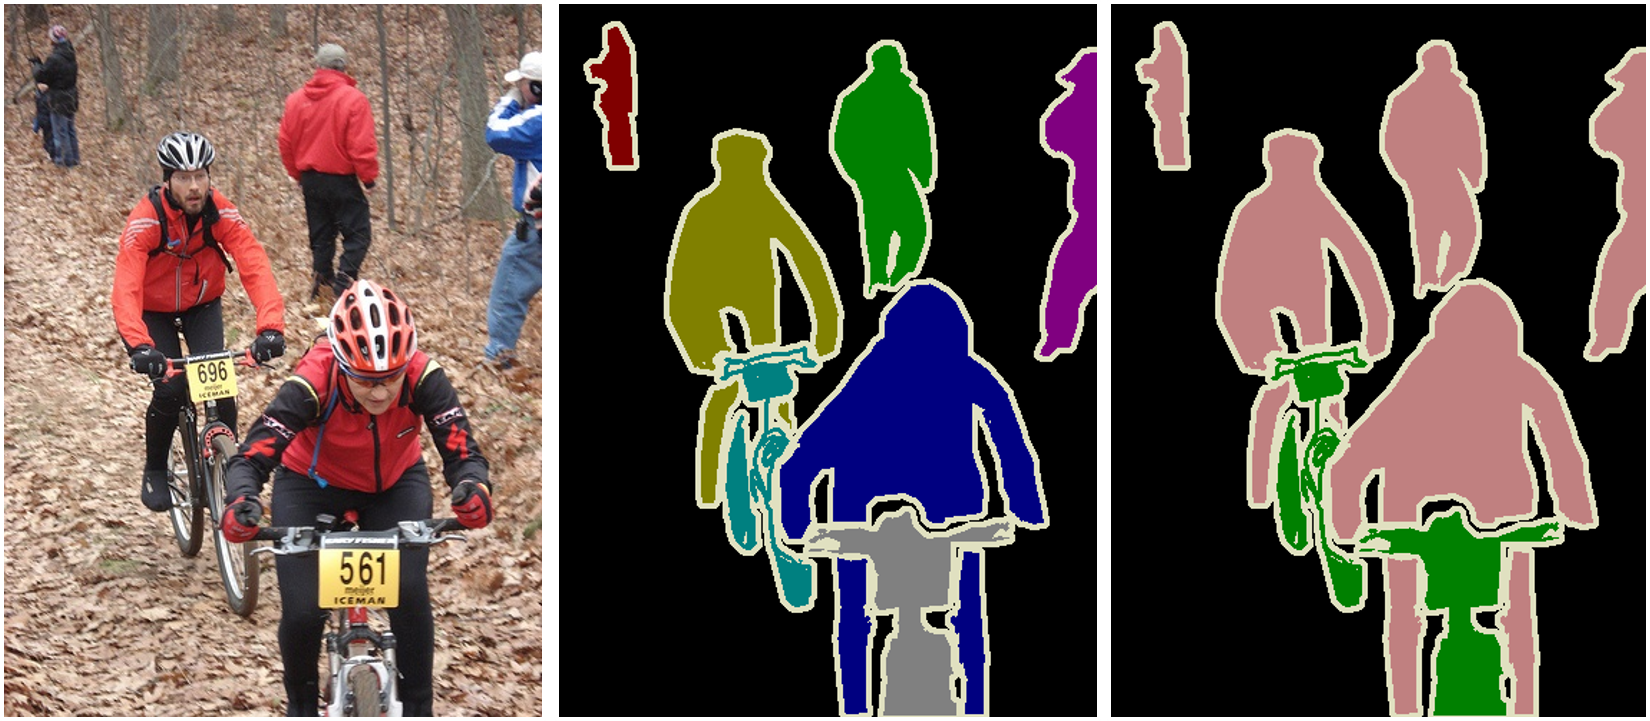
\includegraphics[width=\textwidth]{semantic_image_segmentation}
    \captionsource
    {Semantic segmentation: example image (left), object segmentation (middle), semantic image segmentation (right)}
    {The PASCAL Visual Object Classes \cite{voc}}
     \label{fig:semantic_image_segmentation}
\end{figure}

Understanding what objects are present on an image is a key issue in a large variety of practical applications which require image processing. One of the possible uses of semantic image segmentation is in the automotive industry. Thanks to road segmentation, which include obstacle detection and classification, autonomous driving may be possible. It is also applicable to traffic control systems, or smart parking solutions. Similarly, it is needed for robot vision in order to allow decision making based on what is in a field of view of a robot.  Furthermore, semantic image segmentation is required for recognition systems for example to provide access to a restricted area based on people biometric features. Similarly, a large set of applications for object recognition and classification is connected with medical imaging, as scanning results are in a form of a substantial number of images, which then have to be analysed by a doctor. Thanks to automatic detection tools, for example to locate tissue pathologies from images, diagnosis can be much easier and less time-consuming.  Those are only a few examples of possible applications for semantic image segmentation, however, all of them have one thing in common – they require high precision and accuracy of the results, which can be achieved using various techniques. 
 
